\section[Routing Model Results]{Evaluation of the Medical Image Routing Model}

The medical image routing model represents the first level of the proposed hierarchical diagnostic framework and therefore plays a critical role in determining the overall effectiveness of the system. Since all incoming images must first pass through the routing stage before being analyzed by specialized diagnostic models, the reliability of this component directly impacts the performance of the entire framework. Consequently, a comprehensive evaluation was conducted to assess the ability of the routing model to accurately distinguish between chest X-ray images, chest CT scan images, and out-of-distribution images categorized as \emph{Other}.

The evaluation process was designed not only to measure the classification performance of the final selected model but also to compare multiple candidate architectures and investigate the effect of hyperparameter selection on model performance. In particular, several deep learning architectures were trained and evaluated under identical experimental conditions, including a custom convolutional neural network, ResNet50, DenseNet121, and EfficientNetB3. The objective was to identify the architecture that offered the best combination of classification accuracy, generalization capability, and computational efficiency for the image routing task.

\subsection{Implementation Environment and Development Tools}

The routing model was implemented using the Python programming language and developed within a Jupyter Notebook environment. The deep learning pipeline was built using TensorFlow version 2.20.0 and Keras version 3.12.0, which provided the necessary functionality for constructing, training, and evaluating convolutional neural networks. Data preprocessing, dataset partitioning, performance evaluation, and metric computation were performed using Scikit-learn version 1.8.0.

Model training and experimentation were conducted on a workstation equipped with an NVIDIA RTX 2060 graphics processing unit (GPU). The availability of GPU acceleration significantly reduced training times and enabled the efficient evaluation of multiple candidate architectures and hyperparameter configurations. Table~\ref{tab:routing_tools} summarizes the software and hardware environment used during the implementation and evaluation process.

\begin{table}[H]
	\centering
	\caption{Software and hardware environment used for implementing the routing model.}
	\label{tab:routing_tools}
	\begin{tabular}{|l|l|}
		\hline
		\textbf{Component} & \textbf{Specification} \\
		\hline
		Programming Language & Python 3.12 \\
		\hline
		Deep Learning Framework & TensorFlow 2.20.0 \\
		\hline
		Neural Network API & Keras 3.12.0 \\
		\hline
		Machine Learning Library & Scikit-learn 1.8.0 \\
		\hline
		Development Environment & Jupyter Notebook \\
		\hline
		GPU & NVIDIA RTX 2060 \\
		\hline
	\end{tabular}
\end{table}

\subsection{Dataset Preparation and Experimental Setup}

The aggregated routing dataset consisted of three image categories corresponding to the target classes of the routing problem. The first category contained chest X-ray images, the second category contained chest CT scan images, and the third category consisted of out-of-distribution images grouped under the \emph{Other} class. The final dataset contained a total of 19,615 images distributed across the three classes as shown in Table~\ref{tab:routing_dataset_distribution}.

\begin{figure}[H]
	\centering
	
	% ---------------- LEFT: TABLE ----------------
	\begin{minipage}[c]{0.46\textwidth}
		\centering
		
		\captionof{table}{Class distribution of the routing dataset.}
		\label{tab:routing_dataset_distribution}
		
		\vspace{0.3cm}
		
		\begin{tabular}{|l|c|}
			\hline
			\textbf{Class} & \textbf{Number of Images} \\
			\hline
			Chest X-Ray & 7,123 \\
			\hline
			Chest CT Scan & 2,534 \\
			\hline
			Other & 9,958 \\
			\hline
			Total & 19,615 \\
			\hline
		\end{tabular}
		
	\end{minipage}
	\hfill
	% ---------------- RIGHT: FIGURE ----------------
	\begin{minipage}[c]{0.46\textwidth}
		\centering
		
		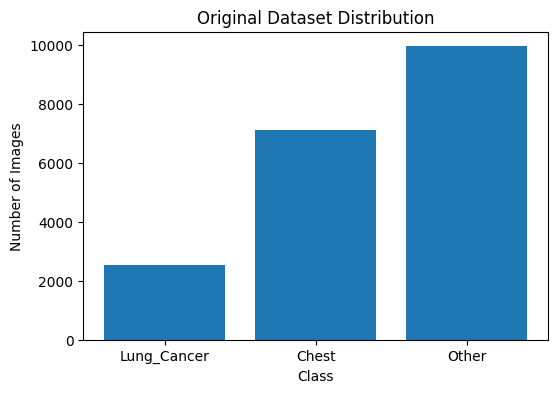
\includegraphics[
		width=\linewidth
		]{assets/dataset_dist_rm.png}
		
		\captionof{figure}{Distribution of the routing dataset classes.}
		\label{fig:routing_dataset_distribution}
		
	\end{minipage}
	
	\caption{Summary of the routing dataset distribution.}
	\label{fig:routing_dataset_summary}
\end{figure}

To ensure a fair evaluation procedure, the dataset was partitioned using a stratified sampling strategy. This approach preserved the original class distribution across all subsets and prevented sampling bias from influencing the evaluation results. The dataset was divided into training, validation, and testing subsets using a ratio of 70\%, 15\%, and 15\%, respectively.

A number of techniques were employed to mitigate the effects of class imbalance. First, class weights were incorporated during training to increase the contribution of minority classes to the optimization process. Second, stratified sampling was utilized to preserve representative class distributions across all dataset splits. Third, extensive data augmentation was applied to improve generalization and increase sample diversity. The augmentation pipeline included common image transformation techniques such as rotation, translation, zooming, flipping, brightness adjustment, and contrast variation. Geometric transformations that could significantly distort medical structures, such as excessive shearing, were intentionally avoided in order to preserve clinically relevant image features.

All models were trained using a batch size of 8 for a total of 10 epochs. The same training, validation, and testing partitions were used across all experiments to ensure consistency when comparing model performance.

\subsection{Learning Rate Optimization}

Since learning rate selection plays a crucial role in determining convergence behavior and final model performance, multiple learning rate values were investigated for each architecture. The evaluated learning rates included \(10^{-5}\), \(10^{-4}\), \(10^{-3}\), and \(10^{-2}\).

The experiments revealed that different architectures exhibited different optimization characteristics. DenseNet121 and ResNet50 achieved their highest performance when trained using a learning rate of \(10^{-2}\), whereas EfficientNetB3 performed best with a learning rate of \(10^{-4}\). Due to its relatively shallow architecture and limited feature extraction capacity, the custom convolutional neural network achieved its best results with a learning rate of \(10^{-5}\).

Table~\ref{tab:learning_rates} summarizes the optimal learning rate selected for each evaluated architecture.

\begin{table}[H]
	\centering
	\caption{Optimal learning rates identified during hyperparameter tuning.}
	\label{tab:learning_rates}
	\begin{tabular}{|l|c|}
		\hline
		\textbf{Model} & \textbf{Optimal Learning Rate} \\
		\hline
		Custom CNN & $10^{-5}$ \\
		\hline
		ResNet50 & $10^{-2}$ \\
		\hline
		DenseNet121 & $10^{-2}$ \\
		\hline
		EfficientNetB3 & $10^{-4}$ \\
		\hline
	\end{tabular}
\end{table}

These findings highlight the importance of architecture-specific hyperparameter tuning. Applying a common learning rate across all models would have resulted in suboptimal performance and potentially misleading comparisons between candidate architectures.

\subsection{Comparative Evaluation of Candidate Architectures}

To identify the most suitable backbone architecture for the routing model, four candidate architectures were trained and evaluated under identical conditions. The evaluated architectures included a custom CNN developed specifically for this task, ResNet50, DenseNet121, and EfficientNetB3.

The comparison focused on commonly used classification metrics, including accuracy, precision, recall, F1-score, and loss. Table~\ref{tab:routing_model_comparison} summarizes the performance of all evaluated architectures.

\begin{table}[H]
	\centering
	\caption{Performance comparison of candidate routing architectures.}
	\label{tab:routing_model_comparison}
	\begin{tabular}{|l|c|c|c|c|c|}
		\hline
		\textbf{Model} &
		\textbf{Accuracy} &
		\textbf{Precision} &
		\textbf{Recall} &
		\textbf{F1-Score} &
		\textbf{Loss} \\
		\hline
		Custom CNN & 1.0000 & 1.0000 & 1.0000 & 1.0000 & 0.0011 \\
		\hline
		ResNet50 & 1.0000 & 1.0000 & 1.0000 & 1.0000 & $1.782 \times 10^{-6}$ \\
		\hline
		EfficientNetB3 & 1.0000 & 1.0000 & 1.0000 & 1.0000 & $1.9816 \times 10^{-5}$ \\
		\hline
		DenseNet121 & 1.0000 & 1.0000 & 1.0000 & 1.0000 & $1.5126 \times 10^{-7}$ \\
		\hline
	\end{tabular}
\end{table}

The results demonstrate the superiority of DenseNet121 for the routing task. DenseNet121 achieved perfect classification performance on the test dataset, obtaining an accuracy, precision, recall, and F1-score of 100\%. Furthermore, the model achieved an extremely low loss value of \(1.5126 \times 10^{-7}\), indicating highly confident predictions and excellent convergence behavior.

The dense connectivity mechanism employed by DenseNet121 enables efficient feature reuse throughout the network and facilitates gradient propagation across deep layers. As a result, the model was able to learn highly discriminative representations that effectively separated the three image categories. Based on these findings, DenseNet121 was selected as the backbone architecture of the final routing model.

\begin{figure}[htbp]
	\centering
	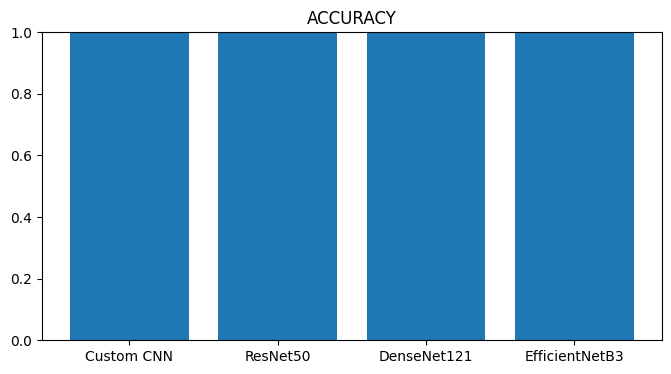
\includegraphics[width=\linewidth]{assets/models_acc_rm.png}
	\caption{Comparison of classification accuracy across all evaluated routing architectures.}
	\label{fig:routing_accuracy_comparison}
\end{figure}

\subsection{Training and Validation Behavior}

In addition to evaluating final classification performance, the training dynamics of each architecture were analyzed to assess convergence behavior and learning stability throughout the optimization process.

Figures~\ref{fig:routing_training_curves} illustrate the evolution of training accuracy, validation accuracy, training loss, and validation loss during the training process for all evaluated models.

\begin{figure}[htbp]
	\centering
	
	% -------------------------------------------------
	% Custom CNN
	% -------------------------------------------------
	\begin{subfigure}{0.95\textwidth}
		\centering
		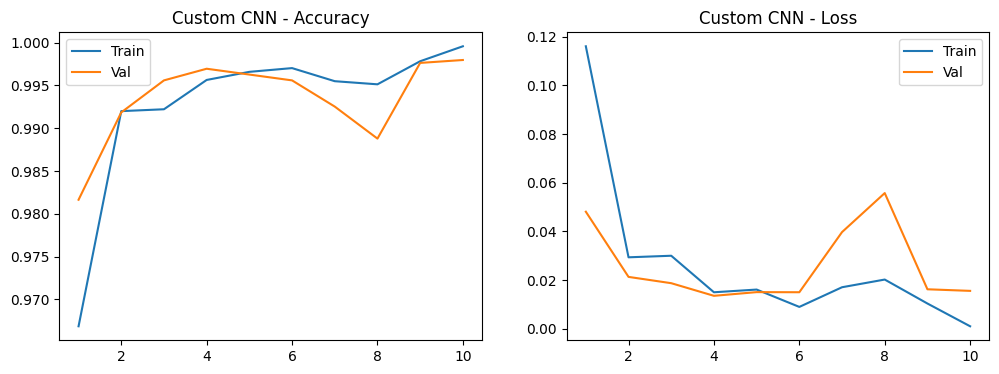
\includegraphics[
		width=\linewidth,
		height=0.18\textheight,
		keepaspectratio
		]{assets/curve_customcnn.png}
		\caption{Training and validation curves for the Custom CNN model.}
		\label{fig:customcnn_training_curves}
	\end{subfigure}
	
	\vspace{0.25cm}
	
	% -------------------------------------------------
	% ResNet50
	% -------------------------------------------------
	\begin{subfigure}{0.95\textwidth}
		\centering
		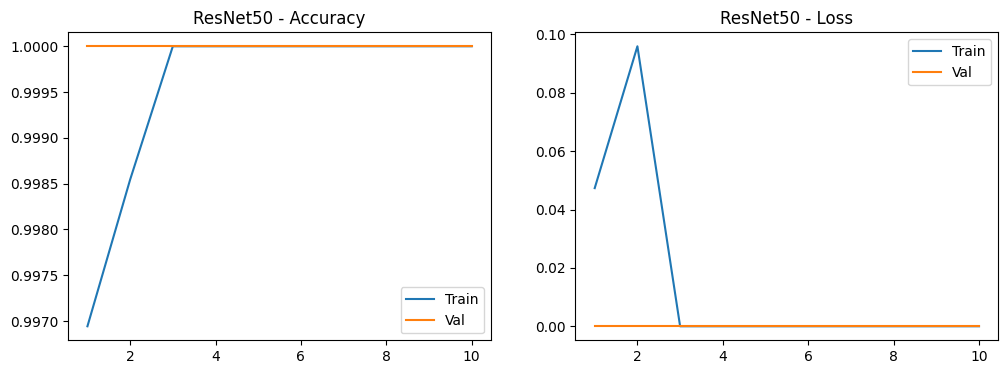
\includegraphics[
		width=\linewidth,
		height=0.18\textheight,
		keepaspectratio
		]{assets/curve_resnet.png}
		\caption{Training and validation curves for the ResNet50 model.}
		\label{fig:resnet50_training_curves}
	\end{subfigure}
	
	\vspace{0.25cm}
	
	% -------------------------------------------------
	% EfficientNetB3
	% -------------------------------------------------
	\begin{subfigure}{0.95\textwidth}
		\centering
		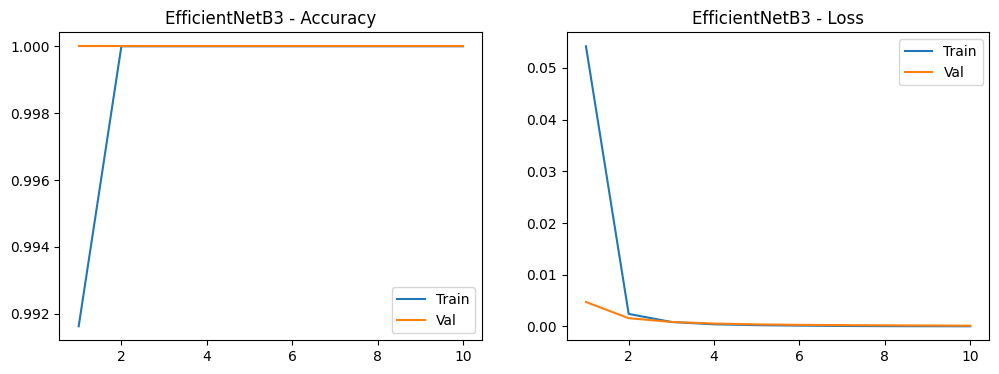
\includegraphics[
		width=\linewidth,
		height=0.18\textheight,
		keepaspectratio
		]{assets/curve_efficient.png}
		\caption{Training and validation curves for the EfficientNetB3 model.}
		\label{fig:efficientnet_training_curves}
	\end{subfigure}
	
	\vspace{0.25cm}
	
	% -------------------------------------------------
	% DenseNet121
	% -------------------------------------------------
	\begin{subfigure}{0.95\textwidth}
		\centering
		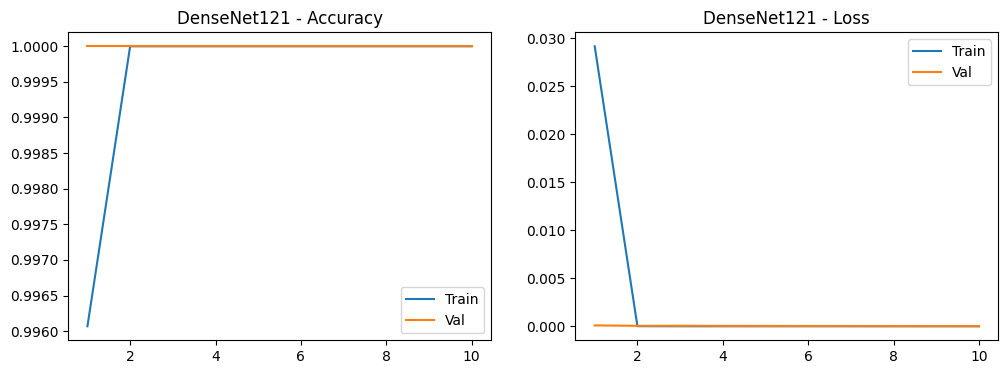
\includegraphics[
		width=\linewidth,
		height=0.18\textheight,
		keepaspectratio
		]{assets/curve_densenet.png}
		\caption{Training and validation curves for the DenseNet121 model.}
		\label{fig:densenet121_training_curves}
	\end{subfigure}
	
	\caption{Training and validation performance curves for all evaluated routing model architectures. Each figure illustrates the evolution of accuracy and loss throughout the training process and provides insight into model convergence, optimization stability, and generalization behavior.}
	\label{fig:routing_training_curves}
\end{figure}

Analysis of these curves provides valuable insight into convergence speed, optimization stability, and generalization behavior. The results indicate that DenseNet121 exhibited rapid convergence while maintaining stable validation performance throughout training, further supporting its selection as the final routing architecture.

\subsection{Confusion Matrix Analysis}

To further investigate classification performance, confusion matrices were generated for each evaluated architecture. Confusion matrices provide a detailed view of model predictions by illustrating the relationship between true class labels and predicted class labels.

The confusion matrix analysis is particularly important for the routing stage because misclassification at this level may cause images to be forwarded to an inappropriate downstream diagnostic model. Therefore, minimizing routing errors is essential for ensuring the reliability of the entire hierarchical framework.

Figure~\ref{fig:all_confusion_matrices} presents the confusion matrices obtained for all evaluated architectures.

\begin{figure}[htbp]
	\centering
	
	% ---------------- Row 1 ----------------
	\begin{subfigure}[t]{0.48\textwidth}
		\centering
		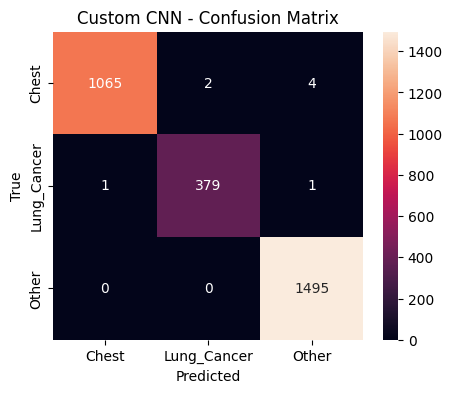
\includegraphics[
		width=\linewidth,
		height=0.28\textheight,
		keepaspectratio
		]{assets/customcnn_cm_rm.png}
		\caption{Custom CNN}
	\end{subfigure}
	\hfill
	\begin{subfigure}[t]{0.48\textwidth}
		\centering
		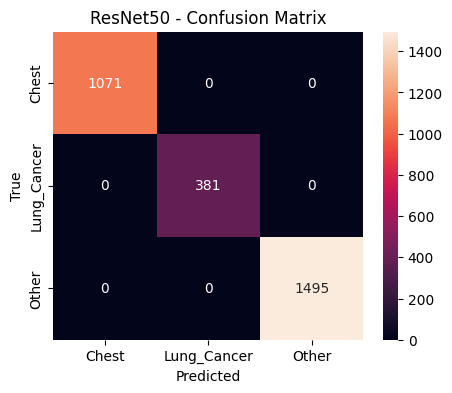
\includegraphics[
		width=\linewidth,
		height=0.28\textheight,
		keepaspectratio
		]{assets/resnet50_cm_rm.png}
		\caption{ResNet50}
	\end{subfigure}
	
	\vspace{0.3cm}
	
	% ---------------- Row 2 ----------------
	\begin{subfigure}[t]{0.48\textwidth}
		\centering
		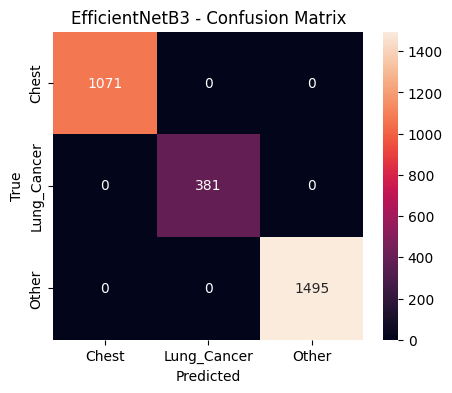
\includegraphics[
		width=\linewidth,
		height=0.28\textheight,
		keepaspectratio
		]{assets/efficient_cm_rm.png}
		\caption{EfficientNetB3}
	\end{subfigure}
	\hfill
	\begin{subfigure}[t]{0.48\textwidth}
		\centering
		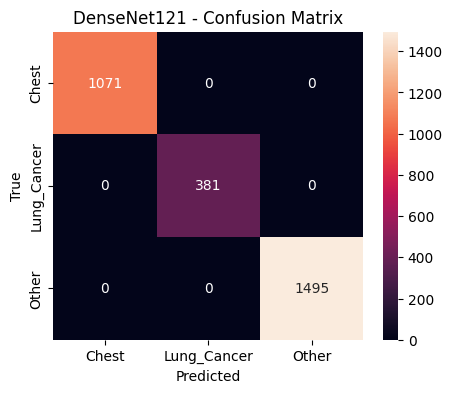
\includegraphics[
		width=\linewidth,
		height=0.28\textheight,
		keepaspectratio
		]{assets/densenet_cm_rm.png}
		\caption{DenseNet121}
	\end{subfigure}
	
	\caption{Confusion matrices for all evaluated routing models across the three classes.}
	\label{fig:all_confusion_matrices}
\end{figure}

The confusion matrix corresponding to DenseNet121 demonstrated perfect classification performance across all three classes, with no observed misclassifications in the test set. This result confirms the model's ability to accurately distinguish between chest X-ray images, chest CT scans, and out-of-distribution images, making it highly suitable for deployment as the first-level routing component within the proposed framework.

\subsection{Discussion}

The experimental results demonstrate that the proposed routing model successfully fulfills its intended objective of accurately identifying image modalities and directing images toward the appropriate diagnostic pathway. The combination of transfer learning, data augmentation, class weighting, and hyperparameter optimization enabled the evaluated architectures to achieve strong classification performance despite the inherent challenges associated with heterogeneous medical imaging data.

Among all tested architectures, DenseNet121 consistently produced the most favorable results and achieved perfect performance on the test dataset. The model's dense connectivity structure enabled efficient feature reuse and facilitated the extraction of highly discriminative modality-specific representations. Furthermore, the confusion matrix analysis confirmed the absence of routing errors, indicating that all images were successfully assigned to their correct categories.

These findings validate the effectiveness of the proposed first-level routing strategy and demonstrate that the routing component provides a reliable foundation for the subsequent disease classification and lung cancer detection stages of the overall framework.